\begin{figure*}[t]
    \centering
    % --- WS ---
    \subfloat[SW ($n=4$)]{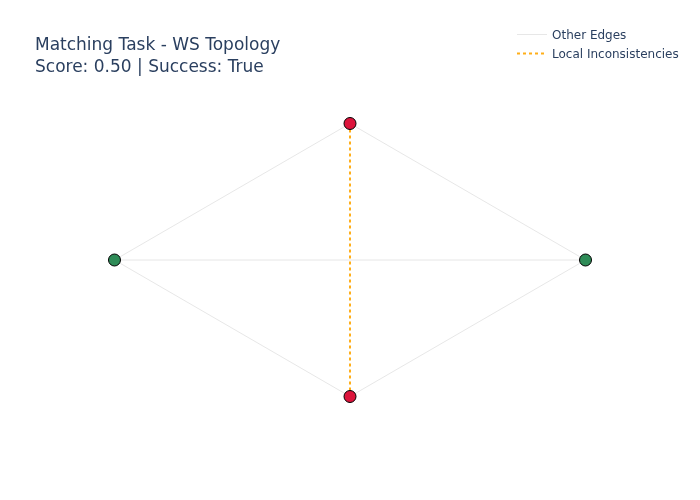
\includegraphics[trim=100 100 90 100,clip,width=0.12\textwidth]{figures/topology/matching_results_20250917_224359_rounds8_gpt-4o-mini_nodes4_langgraph_matching_original.png}}
    \subfloat[SW ($n=8$)]{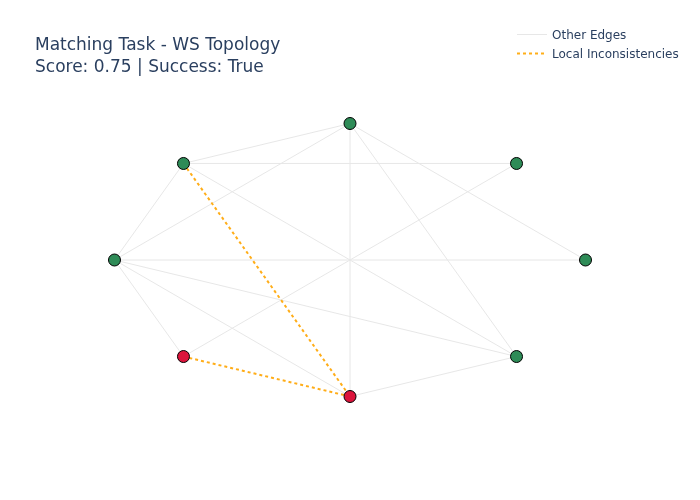
\includegraphics[trim=100 100 90 100,clip,width=0.16\textwidth]{figures/topology/matching_results_20250917_224622_rounds8_gpt-4o-mini_nodes8_langgraph_matching_original.png}}
    \subfloat[SW ($n=16$)]{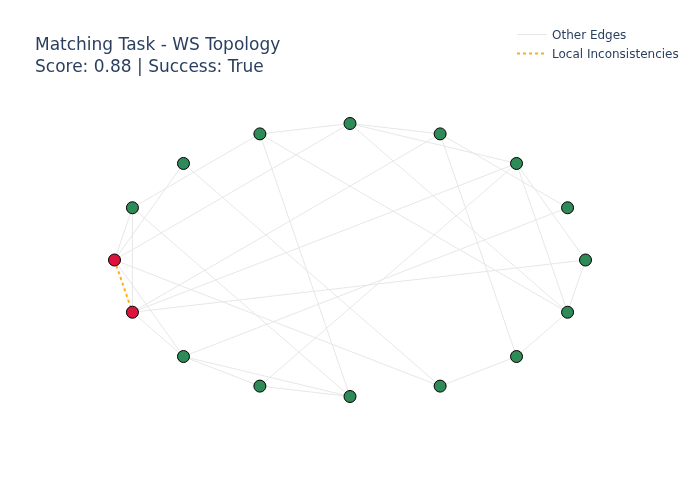
\includegraphics[trim=100 100 90 100,clip,width=0.19\textwidth]{figures/topology/matching_results_20250917_224907_rounds8_gpt-4o-mini_nodes16_langgraph_matching_original.png}}
    \subfloat[SW ($n=50$)]{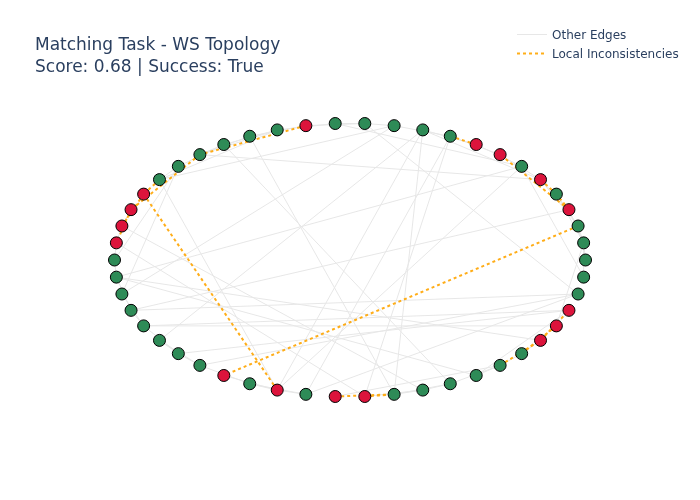
\includegraphics[trim=100 100 90 100,clip,width=0.22\textwidth]{figures/topology/matching_results_20250920_223026_rounds11_gpt-4o-mini_nodes50_langgraph_matching_original.png}}
    \subfloat[SW ($n=100$)]{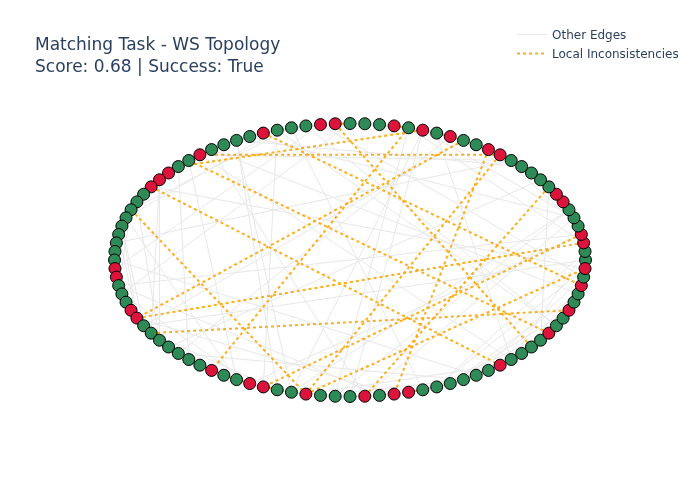
\includegraphics[trim=100 100 90 100,clip,width=0.26\textwidth]{figures/topology/matching_results_20250919_123428_rounds15_gpt-4o-mini_nodes100_langgraph_matching_original.png}}
    \\
    \vspace{2mm}
    % --- BA ---
    \subfloat[SF ($n=4$)]{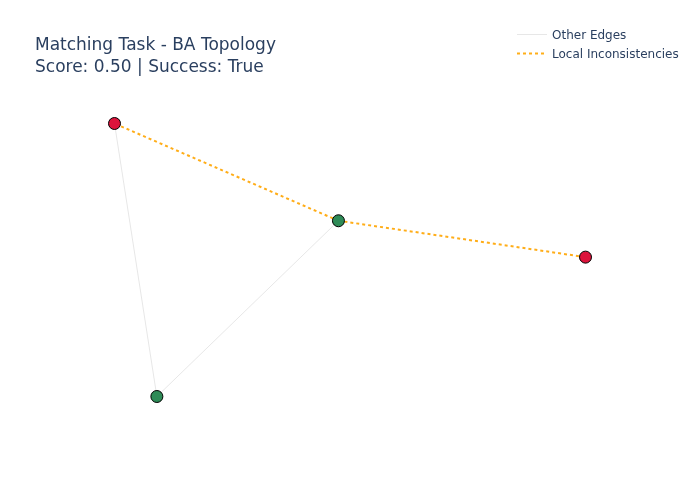
\includegraphics[trim=100 100 90 100,clip,width=0.12\textwidth]{figures/topology/matching_results_20250917_225048_rounds8_gpt-4o-mini_nodes4_langgraph_matching_original.png}}
    \subfloat[SF ($n=8$)]{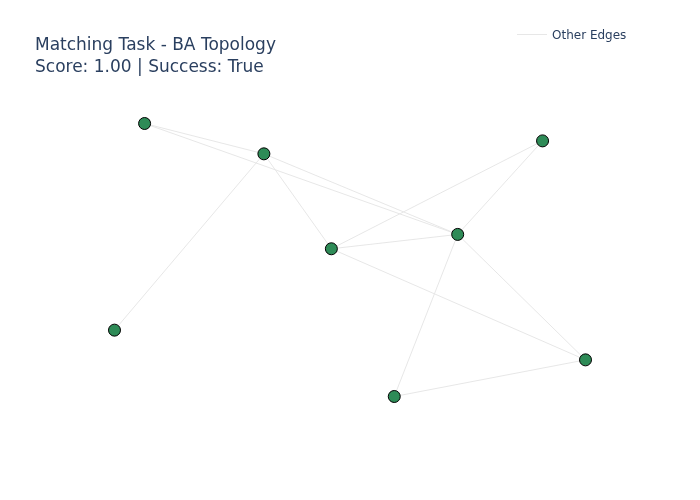
\includegraphics[trim=100 100 90 100,clip,width=0.16\textwidth]{figures/topology/matching_results_20250917_225237_rounds8_gpt-4o-mini_nodes8_langgraph_matching_original.png}}
    \subfloat[SF ($n=16$)]{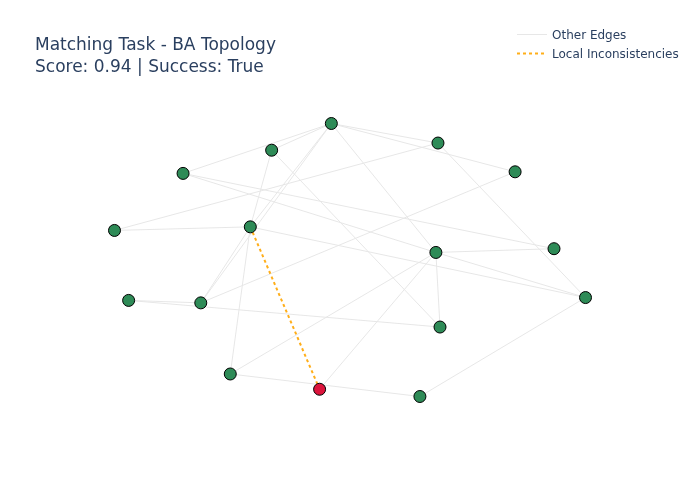
\includegraphics[trim=100 100 90 100,clip,width=0.19\textwidth]{figures/topology/matching_results_20250917_225456_rounds8_gpt-4o-mini_nodes16_langgraph_matching_original.png}}
    \subfloat[SF ($n=50$)]{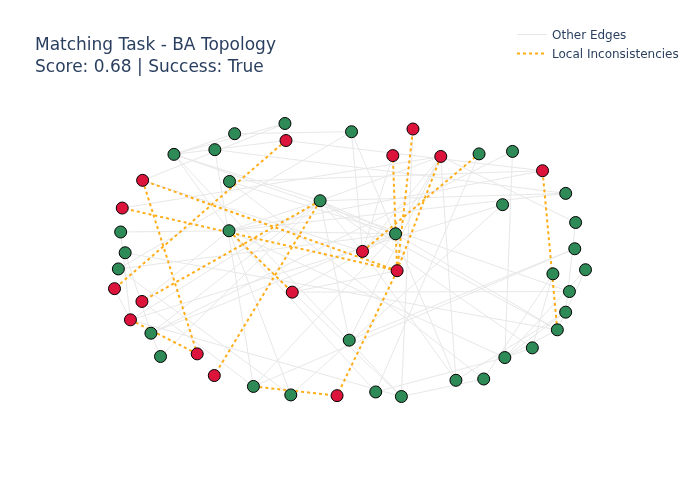
\includegraphics[trim=100 100 90 100,clip,width=0.22\textwidth]{figures/topology/matching_results_20250920_180551_rounds11_gpt-4o-mini_nodes50_langgraph_matching_original.png}}
    \subfloat[SF ($n=100$)]{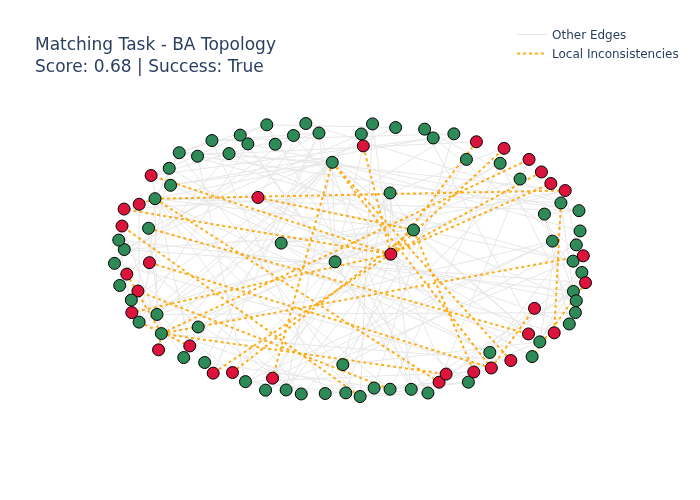
\includegraphics[trim=100 100 90 100,clip,width=0.26\textwidth]{figures/topology/matching_results_20250920_181618_rounds11_gpt-4o-mini_nodes100_langgraph_matching_original.png}}
    \\
    \vspace{2mm}
    % --- DT ---
    \subfloat[DT ($n=4$)]{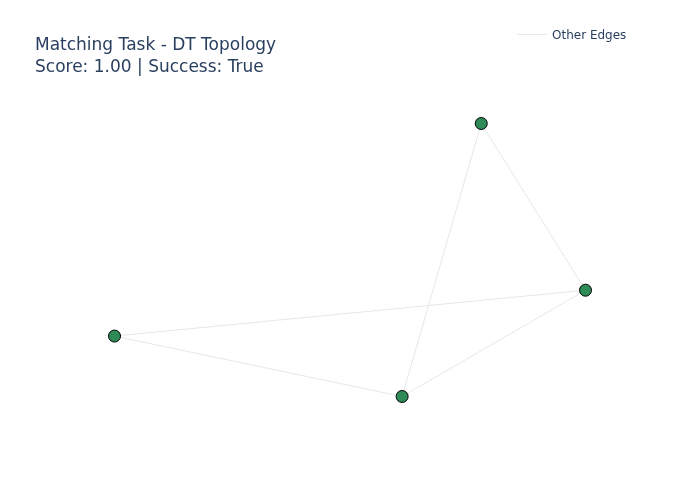
\includegraphics[trim=100 100 90 100,clip,width=0.12\textwidth]{figures/topology/matching_results_20250917_225625_rounds8_gpt-4o-mini_nodes4_langgraph_matching_original.png}}
    \subfloat[DT ($n=8$)]{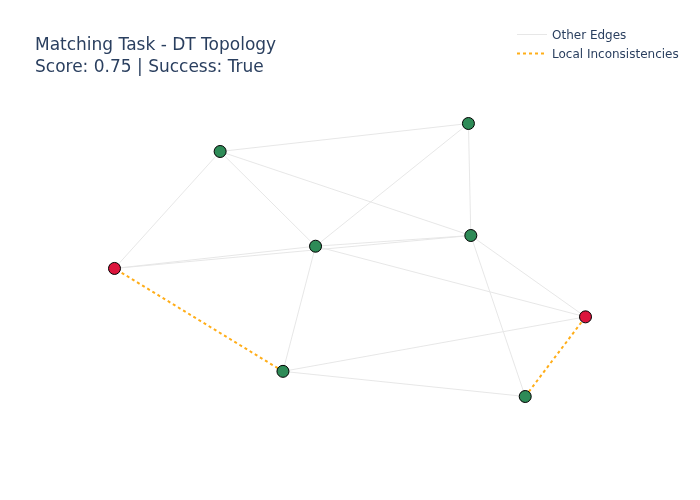
\includegraphics[trim=100 100 90 100,clip,width=0.16\textwidth]{figures/topology/matching_results_20250917_225759_rounds8_gpt-4o-mini_nodes8_langgraph_matching_original.png}}
    \subfloat[DT ($n=16$)]{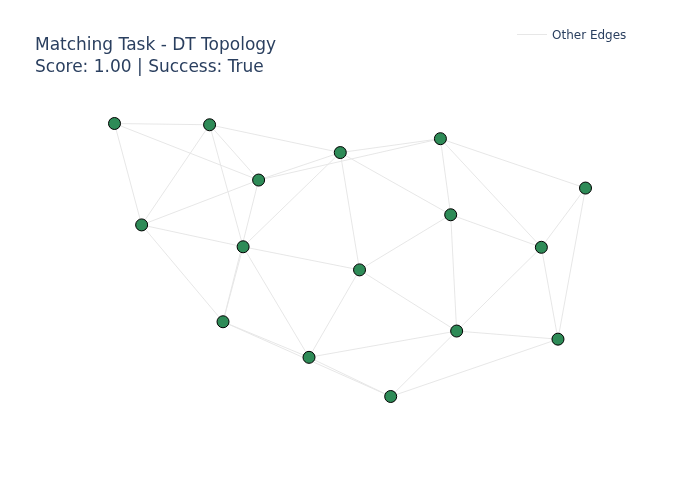
\includegraphics[trim=100 100 90 100,clip,width=0.19\textwidth]{figures/topology/matching_results_20250917_230008_rounds8_gpt-4o-mini_nodes16_langgraph_matching_original.png}}
    \subfloat[DT ($n=50$)]{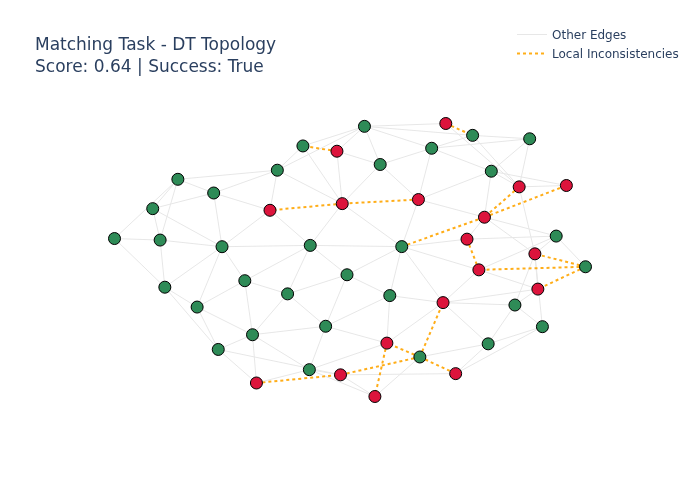
\includegraphics[trim=100 100 90 100,clip,width=0.22\textwidth]{figures/topology/matching_results_20250920_182438_rounds13_gpt-4o-mini_nodes50_langgraph_matching_original.png}}
    \subfloat[DT ($n=100$)]{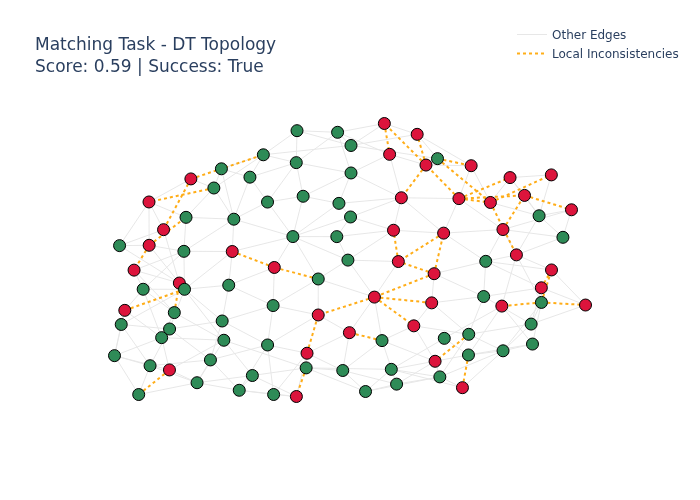
\includegraphics[trim=100 100 90 100,clip,width=0.26\textwidth]{figures/topology/matching_results_20250920_184622_rounds19_gpt-4o-mini_nodes100_langgraph_matching_original.png}}
    \\
    \vspace{2mm}
    % --- SEQUENTIAL ---
    \subfloat[Seq. ($n=4$)]{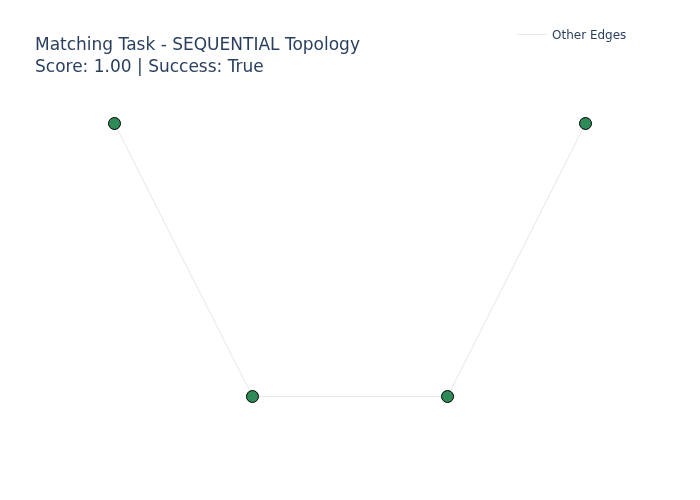
\includegraphics[trim=100 100 90 100,clip,width=0.12\textwidth]{figures/topology/matching_results_20250924_134419_rounds8_gpt-4o-mini_nodes4_crewai-sequential_matching_original.png}}
    \subfloat[Seq. ($n=8$)]{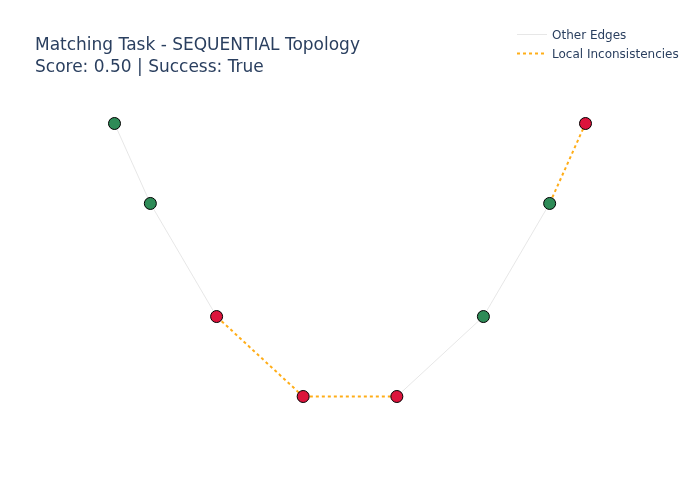
\includegraphics[trim=100 100 90 100,clip,width=0.16\textwidth]{figures/topology/matching_results_20250924_134606_rounds8_gpt-4o-mini_nodes8_crewai-sequential_matching_original.png}}
    \subfloat[Seq. ($n=16$)]{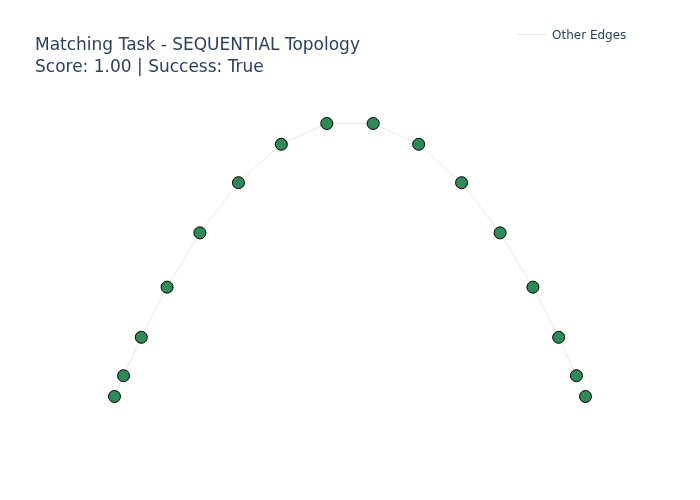
\includegraphics[trim=100 100 90 100,clip,width=0.19\textwidth]{figures/topology/matching_results_20250924_134833_rounds8_gpt-4o-mini_nodes16_crewai-sequential_matching_original.png}}
    \subfloat{\rule{0.22\textwidth}{0pt}} % placeholder without number
    \subfloat{\rule{0.26\textwidth}{0pt}} % placeholder without number
    \\
    \vspace{2mm}
    % --- HIERARCHICAL ---
    \subfloat[Hier. ($n=4$)]{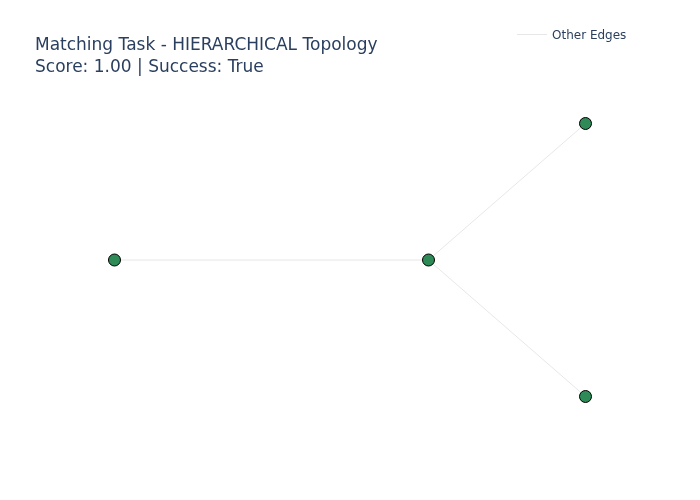
\includegraphics[trim=100 100 90 100,clip,width=0.12\textwidth]{figures/topology/matching_results_20250924_144228_rounds8_gpt-4o-mini_nodes4_crewai-hierarchical_matching_original.png}}
    \subfloat[Hier. ($n=8$)]{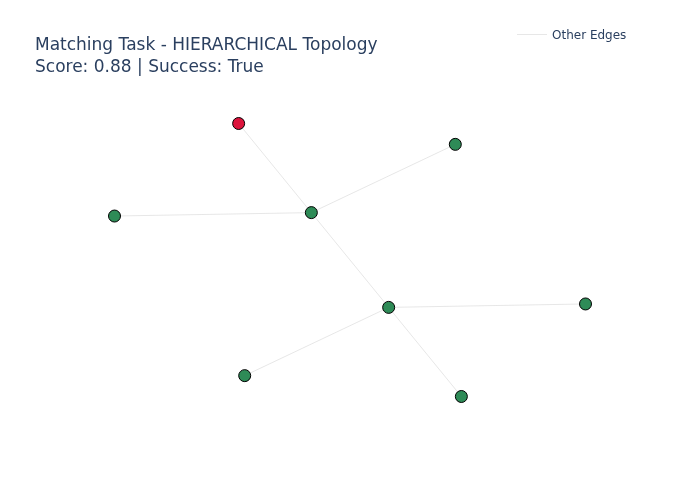
\includegraphics[trim=100 100 90 100,clip,width=0.16\textwidth]{figures/topology/matching_results_20250924_144411_rounds8_gpt-4o-mini_nodes8_crewai-hierarchical_matching_original.png}}
    \subfloat[Hier. ($n=16$)]{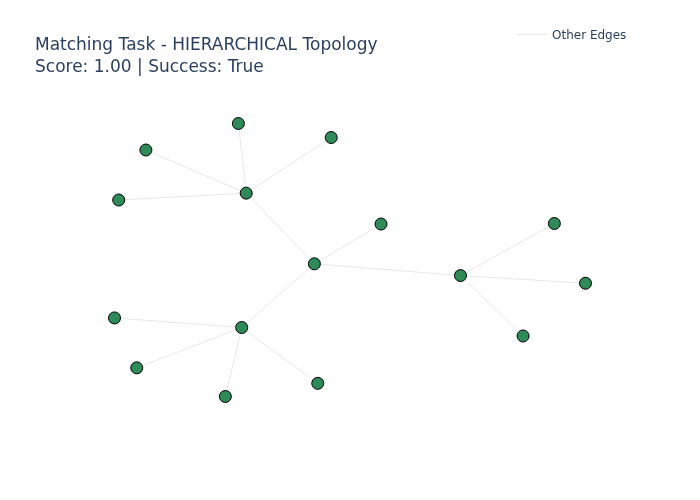
\includegraphics[trim=100 100 90 100,clip,width=0.19\textwidth]{figures/topology/matching_results_20250924_144629_rounds8_gpt-4o-mini_nodes16_crewai-hierarchical_matching_original.png}}
    \subfloat[Hier. ($n=50$)]{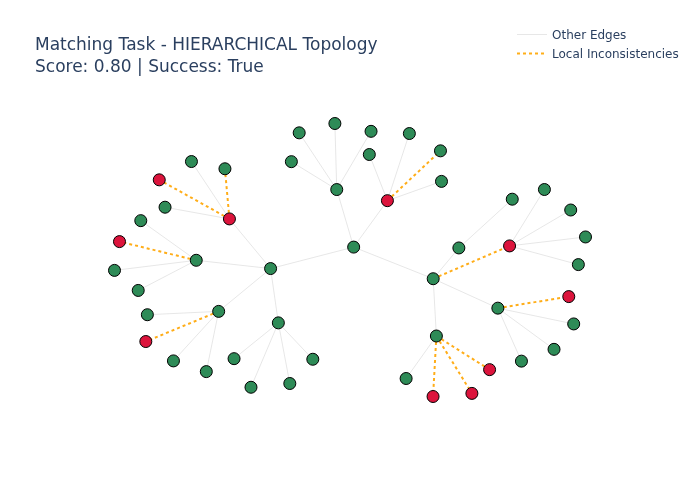
\includegraphics[trim=100 100 90 100,clip,width=0.22\textwidth]{figures/topology/matching_results_20250925_001343_rounds13_gpt-4o-mini_nodes50_crewai-hierarchical_matching_original.png}}
    \subfloat[Hier. ($n=100$)]{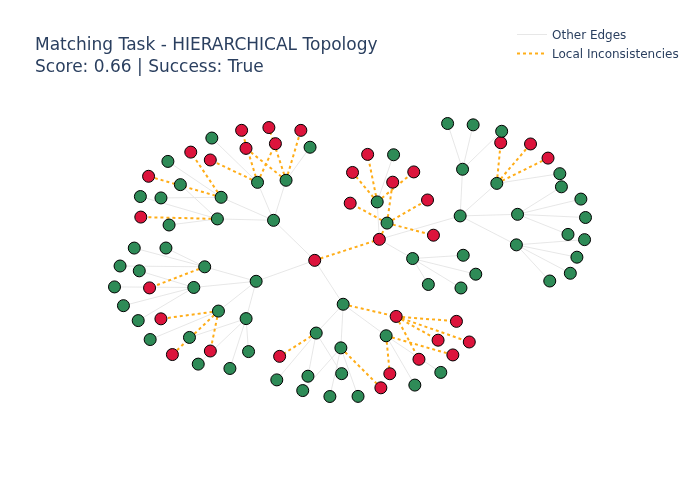
\includegraphics[trim=100 100 90 100,clip,width=0.26\textwidth]{figures/topology/matching_results_20250925_002721_rounds15_gpt-4o-mini_nodes100_crewai-hierarchical_matching_original.png}}
    \\
    \vspace{2mm}
    % --- ALL ---
    \subfloat[All ($n=4$)]{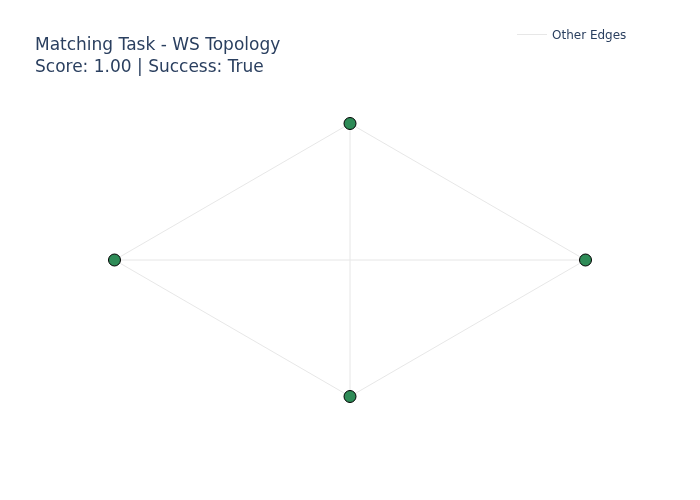
\includegraphics[trim=100 100 90 100,clip,width=0.12\textwidth]{figures/topology/matching_results_20250917_230141_rounds8_gpt-4o-mini_nodes4_concordia_matching_original.png}}
    \subfloat[All ($n=8$)]{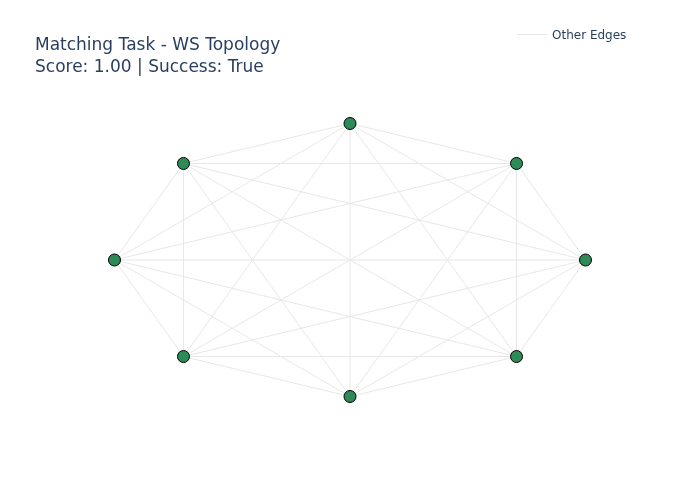
\includegraphics[trim=100 100 90 100,clip,width=0.16\textwidth]{figures/topology/matching_results_20250917_230411_rounds8_gpt-4o-mini_nodes8_concordia_matching_original.png}}
    \subfloat[All ($n=16$)]{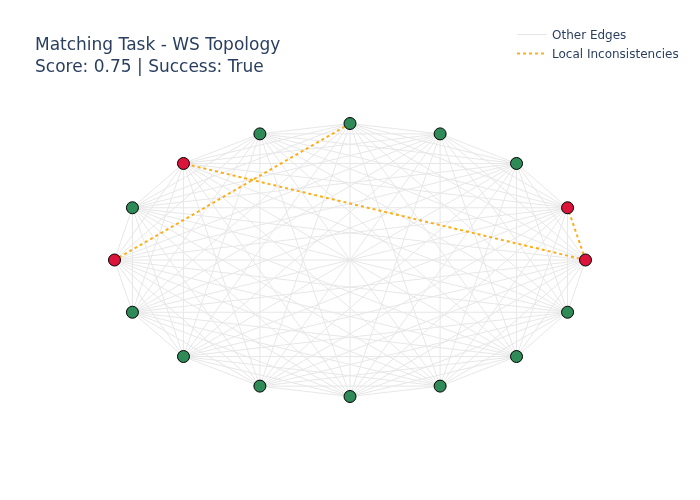
\includegraphics[trim=100 100 90 100,clip,width=0.19\textwidth]{figures/topology/matching_results_20250917_230756_rounds8_gpt-4o-mini_nodes16_concordia_matching_original.png}}
    \subfloat[All ($n=50$)]{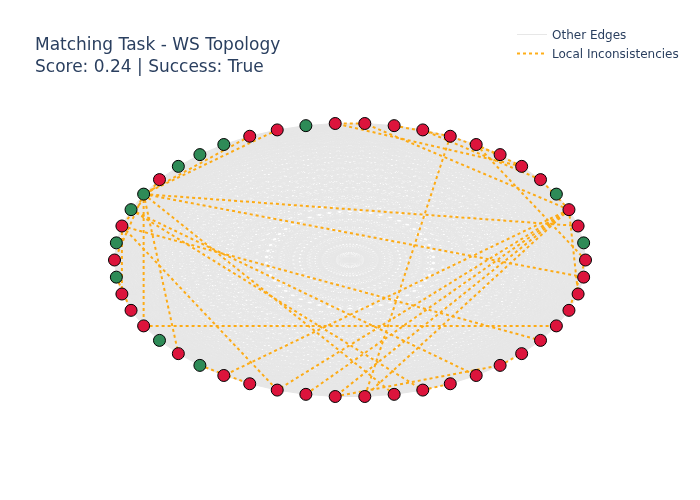
\includegraphics[trim=100 100 90 100,clip,width=0.22\textwidth]{figures/topology/matching_results_20250919_112014_rounds3_gpt-4o-mini_nodes50_concordia_matching_original.png}}
    \subfloat[All ($n=100$)]{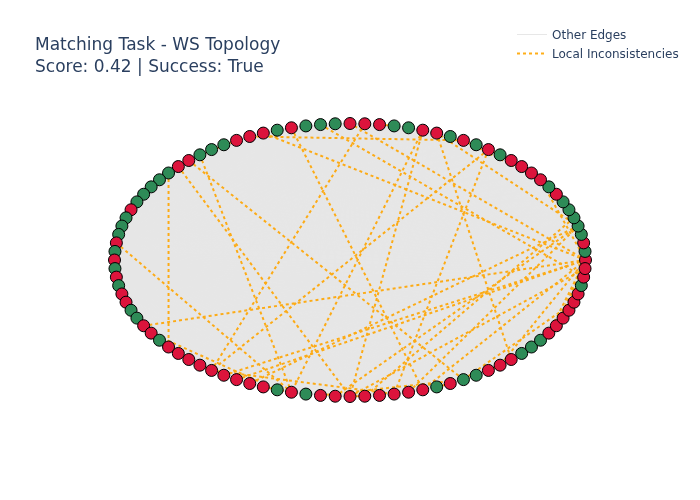
\includegraphics[trim=100 100 90 100,clip,width=0.26\textwidth]{figures/topology/matching_results_20250919_110457_rounds3_gpt-4o-mini_nodes100_concordia_matching_original.png}}
    \\
    \vspace{2mm}
    \caption{Matching experiment outcomes using the \emph{original scoring model}. Each agent selects one of its neighbors (or ``None'') to form a pair. Green nodes denote agents whose selections are locally consistent---that is, they selected a valid neighbor who reciprocated the choice. Red nodes represent agents involved in inconsistencies, such as choosing a non-neighbor, selecting a non-reciprocating partner, or forming idle pairs where both neighbors chose ``None.'' The overall score corresponds to the fraction of locally consistent agents, following the computation described in the text.}


    \label{fig:matching-results}
\end{figure*}
